% Colloquium talk on "A New Method of Solving PDEs" (B. Baccala).
% Audience: general mathematics colloquium.  Target: 50-60 minutes, ~40 slides.
% Frames marked %% OPTIONAL may be cut for a 25-30 minute version;
% doing so leaves roughly 22 slides and a coherent arc.
%
% Build: pdflatex NewMethod-talk.tex  (twice, for the outline/TOC)

\documentclass[10pt,aspectratio=169]{beamer}

\usetheme{metropolis}
\metroset{block=fill, numbering=fraction, progressbar=frametitle}

\usepackage[T1]{fontenc}
\usepackage{amsmath,amssymb,amsthm}
\usepackage{mathtools}
\usepackage{appendixnumberbeamer}
\usepackage{tikz}
\usetikzlibrary{arrows.meta, positioning}

\newcommand{\Pset}{\mathcal{P}}
\newcommand{\Peq}{\mathcal{P}^{=}}
\newcommand{\Pne}{\mathcal{P}^{\neq}}
\newcommand{\C}{\mathbb{C}}
\newcommand{\Q}{\mathbb{Q}}
\newcommand{\Rring}{R}
\newcommand{\cstar}{c^{*}}
\newcommand{\ld}{\operatorname{ld}}

\title{A New Method of Solving PDEs}
\subtitle{Exact non-separable solutions by differential elimination}
\author{Brent Baccala}
\date{\today}

\begin{document}

\maketitle

% ============================================================ HOOK

\begin{frame}{A very well studied equation}
The Schr\"odinger equation for hydrogen, in atomic units:
\[
  -\tfrac{1}{2}\nabla^{2}\Psi \;-\; \tfrac{1}{r}\Psi \;=\; E\,\Psi,
  \qquad r=\sqrt{x^{2}+y^{2}+z^{2}} .
\]

\pause
\alert{The textbook route.} Separate in spherical coordinates,
$\Psi = R(r)\,\Theta(\theta)\,\Phi(\varphi)$, get the radial equation
\[
  r\,\Psi'' + 2\,\Psi' + 2(1+Er)\,\Psi = 0,
\]
and the ground state
\[
  \Psi = e^{-r}, \qquad E = -\tfrac{1}{2}.
\]

\pause
\begin{alertblock}{}
Every solution method here presupposes a \emph{form}: a product, a symmetry, a
transform. What if we let the form be a parameter, and solve for it?
\end{alertblock}
\end{frame}

\begin{frame}{A solution that is not in the textbooks}
The same equation also has the solution
\[
  \boxed{\;\Psi \;=\; J_{0}\!\left(2\sqrt{x+r}\right), \qquad E = 0\;}
\]
where $J_{0}$ is the ordinary Bessel function.

\pause
\begin{itemize}
  \item Not of the separated form $R(r)\Theta(\theta)\Phi(\varphi)$.
  \item Not Cartesian-separable either.
  \item It \emph{is} separable in parabolic coordinates $\xi = r+x$,
        $\eta = r-x$ --- a reflection of hydrogen's hidden $SO(4)$ symmetry.
\end{itemize}

\pause
\bigskip
This was not guessed. It was \alert{computed}, as one of exactly two branches an
algorithm returned.
\end{frame}

\begin{frame}{What this talk is about}
An algorithm that takes

\begin{itemize}
  \item a system of PDEs, as differential polynomials; and
  \item an \alert{ansatz}: a second set of differential polynomials, carrying
        finitely many undetermined constants,
\end{itemize}

and returns \alert{exactly} the values of those constants for which the ansatz
solves the system.

\pause
\bigskip
Three things to take away:
\begin{enumerate}
  \item The reduction to an ODE is organised by \emph{differential-algebraic
        structure}, not by a symmetry or a separation hypothesis.
  \item There is a \alert{completeness theorem}: nothing valid is missed, nothing
        spurious is returned.
  \item The output is a \emph{geometric object} in constant space, not a list of
        solutions.
\end{enumerate}
\end{frame}

\begin{frame}{Outline}
\tableofcontents
\end{frame}

% ============================================================ PART 1

\section{The ansatz}

\begin{frame}{Where this sits}
Exact-solution methods for PDEs each impose a shape:

\medskip
\begin{tabular}{ll}
  separation of variables & $\Psi = X(x)Y(y)Z(z)$ \\[2pt]
  method of characteristics & solution constant along curves \\[2pt]
  transform methods & Fourier, Laplace \\[2pt]
  Lie symmetry / Clarkson--Kruskal & reduction along a symmetry group \\[2pt]
  Green's functions, Duhamel & superposition from a kernel \\
\end{tabular}

\pause
\bigskip
\alert{This method.} Restrict attention to a subset of function space cut out by
finitely many differential polynomials with undetermined constant coefficients,
then \emph{decide} which constants work.

\medskip
Complementary to the above: it presupposes no symmetry of the equation and no
product structure.
\end{frame}

\begin{frame}{The hydrogen ansatz}
Require $\Psi$ to satisfy a \emph{parameterized second-order linear ODE}
\[
  (a_{0}+a_{1}v)\,\frac{d^{2}\Psi}{dv^{2}}
  + (b_{0}+b_{1}v)\,\frac{d\Psi}{dv}
  + (c_{0}+c_{1}v)\,\Psi \;=\; 0
\]
in a single variable $v$, itself a \emph{parameterized combination} of the
coordinates
\[
  v \;=\; v_{1}x + v_{2}y + v_{3}z + v_{4}r .
\]

\pause
Eleven undetermined constants:
\[
  E,\; a_{0}, a_{1},\; b_{0}, b_{1},\; c_{0}, c_{1},\;
  v_{1}, v_{2}, v_{3}, v_{4}\;\in\;\C .
\]

\pause
\begin{alertblock}{The question}
For which $\cstar \in \C^{11}$ does every function satisfying this ansatz satisfy
the PDE?
\end{alertblock}
\end{frame}

\begin{frame}{Two answers, both found by the algorithm}
\begin{columns}[T]
\begin{column}{0.48\textwidth}
\textbf{Branch 1 --- the classical one}
\[
  \begin{gathered}
    a_{1}=v_{4}=1,\quad b_{0}=c_{0}=2 \\
    c_{1}=E,\quad a_{0}=b_{1}=v_{1}=v_{2}=v_{3}=0
  \end{gathered}
\]
gives $v=r$ and the radial equation
\[
  r\Psi''+2\Psi'+2(1+Er)\Psi=0 .
\]
\end{column}
\pause
\begin{column}{0.48\textwidth}
\textbf{Branch 2 --- the other one}
\[
  \begin{gathered}
    E=0,\quad a_{0}=0,\ a_{1}=1 \\
    b_{0}=-1,\ b_{1}=0,\quad c_{0}=-1,\ c_{1}=0 \\
    v_{1}=1,\ v_{2}=v_{3}=0,\ v_{4}=1
  \end{gathered}
\]
gives $v=x+r$ and
\[
  v\Psi'' + \Psi' + \Psi = 0
  \;\Rightarrow\;
  \Psi = J_{0}(2\sqrt{v}).
\]
\end{column}
\end{columns}

\pause
\bigskip
Separation of variables finds the first. Nothing about the ansatz privileges it
over the second.
\end{frame}

% ============================================================ PART 2

\section{Just enough differential algebra}

\begin{frame}{Differential rings}
A \alert{derivation} $\delta$ on a ring: additive, with
$\delta(ab) = \delta(a)b + a\delta(b)$.

\medskip
A \alert{differential ring} is a ring with finitely many commuting derivations
$\Delta = \{\delta_{1},\dots,\delta_{m}\}$.

\pause
\medskip
A \alert{differential ideal} is an ideal closed under every $\delta \in \Delta$.
Write $[S]$ for the differential ideal generated by $S$ --- the ordinary ideal
generated by $S$ \emph{and all its derivatives}.

\pause
\medskip
$\sqrt{I}$ is the \alert{radical}. In characteristic zero it is again a
differential ideal.

\pause
\begin{block}{Why the radical is the right object}
By the Ritt--Raudenbush Nullstellensatz, $\sqrt{[A]}$ is the \emph{vanishing
ideal} of the solution set of $A$. So
\[
  P \in \sqrt{[A]}
  \iff
  \text{$P$ vanishes at every solution of $A$.}
\]
\end{block}
\end{frame}

\begin{frame}{Encoding an ODE as differential polynomials}
We work in a \emph{partial} differential ring but want to impose \emph{ordinary}
differential equations. How?

\pause
\medskip
For an $n$-th order linear ODE in $y(v)$, introduce $n+2$ new indeterminates:
$y, y', \dots, y^{(n)}$ and the independent variable $v$ --- all of them
differential indeterminates of the ambient ring.

\pause
\medskip
Tie them together with chain-rule equations. For $v = v_{1}x + \cdots$:
\[
  \delta_{x} y = y' \,\delta_{x} v, \qquad
  \delta_{x} y' = y'' \,\delta_{x} v, \qquad \dots
\]
and impose the ODE itself as one more differential polynomial.

\pause
\medskip
\alert{Note.} $\Psi'$ and $\Psi''$ are \emph{separate indeterminates}, not
$\Delta$-derivatives of $\Psi$. They are bound to $\Psi$ only by these equations.
\end{frame}

\begin{frame}{Non-polynomial functions are not a limitation}
Most elementary and special functions are solutions of differential polynomials.

\medskip
\begin{tabular}{ll}
  $\cos x,\ \sin x$ & $f'' + f = 0$ \\[3pt]
  $\exp x$          & $g' = g$ \\[3pt]
  $\ln x$           & $h' = 1/x$, i.e.\ $x\,h' = 1$ \\[3pt]
  $J_{0}$           & a second-order linear ODE with polynomial coefficients \\
\end{tabular}

\pause
\bigskip
Introducing $\cos x$ into $\Q[x,y]\{f,f'\}$:
\[
  f_{x} = f', \quad f_{y} = 0, \qquad f'_{x} = -f, \quad f'_{y} = 0 .
\]

\pause
This admits $A\cos x + B\sin x$ --- a solution \emph{space}, not a single
function. That is normal; one pins it down at the end, as one would with a
boundary condition.
\end{frame}

\begin{frame}{Rankings, leaders, reduction}
Fix a \alert{ranking}: a total order on the derivatives with
$u < \delta u$ and $u<v \Rightarrow \delta u < \delta v$.

\pause
\medskip
For a differential polynomial $p$:
\begin{itemize}
  \item its \alert{leader} $u_{p}$ is the highest-ranked derivative appearing;
  \item its \alert{initial} is the leading coefficient in $u_{p}$;
  \item its \alert{separant} is $\partial p / \partial u_{p}$.
\end{itemize}

\pause
\begin{block}{Ritt's full reduction}
Reducing $p$ modulo a set $A$ yields a remainder $r$ and a product $h$ of
initials and separants with
\[
  h\cdot p - r \;\in\; [A],
  \qquad
  r \text{ fully reduced w.r.t.\ } A .
\]
Equivalently $r \in [A] : H_{A}^{\infty}$: a division algorithm, but one that
clears denominators as it goes.
\end{block}
\end{frame}

\begin{frame}{Simple systems and the Thomas decomposition}
A system $S = (S^{=}, S^{\neq})$ of equations \emph{and inequations} is
\alert{differentially simple} when it is
\begin{itemize}
  \item \emph{algebraically simple}: triangular, non-vanishing initials,
        square-free;
  \item \emph{involutive}: every non-multiplicative prolongation reduces to zero;
  \item minimal, with no reducible inequation.
\end{itemize}

\pause
\begin{block}{Differential Thomas decomposition (B\"achler--Gerdt--Lange-Hegermann--Robertz)}
Any differential system decomposes into finitely many differentially simple
systems whose solution sets \alert{partition} the solution set of the original.
\end{block}

\pause
\medskip
Think of it as: split the problem into finitely many well-behaved branches, with
no double counting.
\end{frame}

\begin{frame}{The workhorse}
\begin{block}{Proposition (Robertz)}
Let $S$ be a simple differential system with equations $p_{1},\dots,p_{s}$, let
$E = [p_{1},\dots,p_{s}]$, and let $q$ be the product of the initials and
separants. Then $E : q^{\infty}$ is a \alert{radical} differential ideal, and
\[
  p \in E : q^{\infty}
  \iff
  \text{the pseudo-remainder of $p$ modulo $p_{1},\dots,p_{s}$ is zero.}
\]
\end{block}

\pause
\bigskip
Two features do all the work later:
\begin{itemize}
  \item It is an \alert{equivalence} --- reduction to zero \emph{decides}
        membership, rather than merely certifying it.
  \item Its only hypothesis is \alert{simplicity}. No coherence, regularity or
        characteristic-set condition to verify separately.
\end{itemize}
\end{frame}

% ============================================================ PART 3

\section{The constant loci}

\begin{frame}{The setup}
\begin{itemize}
  \item An \alert{ansatz} $A(\cstar) = \{a_{1}(\cstar),\dots,a_{k}(\cstar)\}$,
        differential polynomials carrying constants $\cstar \in \C^{n}$.
  \item A \alert{target system} $\Pset = (\Peq, \Pne)$: equations
        $P_{1},\dots,P_{t}$ and inequations $Q_{1},\dots,Q_{w}$.
        Write $Q = Q_{1}\cdots Q_{w}$.
\end{itemize}

\pause
\medskip
The inequations are where a problem's \alert{non-degeneracy} conditions live: a
wavefunction not identically zero, a pressure that does not vanish, a constant
required to be non-zero.

\pause
\bigskip
\begin{alertblock}{}
Without them, questions about the ansatz are usually answered by a degenerate
solution of no interest --- most often $\Psi \equiv 0$.
\end{alertblock}
\end{frame}

\begin{frame}{Two loci}
\begin{block}{Existence locus}
\[
  V_{\exists} \;=\;
  \{\, \cstar \in \C^{n} \;:\; 1 \notin [A(\cstar), \Peq] : Q^{\infty} \,\}
\]
The ansatz and the system have \emph{some} common solution respecting the
inequations.
\end{block}

\pause
\begin{block}{Membership locus}
\[
  V_{\forall} \;=\;
  \{\, \cstar \in \C^{n} \;:\; \Peq \subseteq \sqrt{[A(\cstar)]} : Q^{\infty} \,\}
\]
\emph{Every} solution of the ansatz respecting the inequations satisfies the
system.
\end{block}

\pause
\medskip
$V_{\exists}$ is the honest question. $V_{\forall}$ is the computable one --- and
the rest of the talk is about why that trade is worth making.
\end{frame}

\begin{frame}{Why saturate the radical?}
$\sqrt{[A(\cstar)]}$ is the vanishing ideal of the ansatz's solution set. Saturating
it by $Q$ gives the vanishing ideal of the part where $Q$ does not vanish:
\[
  P \in \sqrt{[A(\cstar)]} : Q^{\infty}
  \iff
  \text{$P$ vanishes at every ansatz solution $f$ with $Q(f) \neq 0$.}
\]

\pause
\medskip
So the inequations \alert{guard} the functions quantified over. They do not assert
anything themselves.

\pause
\begin{alertblock}{Without the saturation}
A value of the constants is rejected whenever \emph{any} ansatz solution violates
the system --- including one on a branch the inequations were written to exclude.
\end{alertblock}
\end{frame}

\begin{frame}{The saturation is free}
\begin{block}{Lemma}
Let $I$ be a \alert{radical} ideal, $P$ and $Q$ ring elements. Then
\[
  P \in I : Q^{\infty} \iff QP \in I .
\]
\end{block}

\pause
\emph{Proof.} ($\Leftarrow$) is the definition. ($\Rightarrow$) if $Q^{k}P \in I$
then $(QP)^{k} = (Q^{k}P)\,P^{k-1} \in I$, and $I$ is radical. \hfill$\square$

\pause
\bigskip
\begin{itemize}
  \item A \alert{single} power of $Q$ suffices --- no saturation exponent to search
        for.
  \item Every membership test becomes: reduce $Q\,P_{j}$ instead of $P_{j}$.
  \item The Thomas decomposition still sees \alert{only the ansatz}.
\end{itemize}
\end{frame}

%% OPTIONAL
\begin{frame}{One trap worth naming}
$V_{\forall}$ is satisfied \alert{vacuously} where the ansatz forces $Q$ to
vanish: there are then no guarded solutions for it to constrain, and
$\sqrt{[A(\cstar)]} : Q^{\infty}$ is the whole ring.

\pause
\medskip
So one carries a second condition, the \alert{non-degeneracy locus}
\[
  N_{Q} \;=\; \{\, \cstar \in \C^{n} \;:\; Q \notin \sqrt{[A(\cstar)]} \,\},
\]
saying the guarded solution set is non-empty.

\pause
\medskip
\begin{itemize}
  \item $V_{\forall}$: the system holds on the guarded solution set.
  \item $N_{Q}$: that set is not empty.
  \item Report $V_{\forall} \cap N_{Q}$; and then
        $V_{\forall} \cap N_{Q} \subseteq V_{\exists}$, unconditionally.
\end{itemize}

\pause
\medskip
$\C^{n} \setminus N_{Q}$ is itself a membership locus --- of the single polynomial
$Q$. Same machinery, one extra reduction.
\end{frame}

\begin{frame}{A toy example, worked three ways}
In $\C[t]\{\Psi,c\}$ with $\delta_{t}c = 0$, take the ansatz and system
\[
  A(c) = \{\,\Psi_{tt} - c\,\Psi\,\}, \qquad P = \Psi_{t} - \Psi .
\]

\pause
\begin{itemize}
  \item \textbf{No inequation.} $\Psi\equiv 0$ solves both for every $c$, so
        $V_{\exists} = \C$. The question is vacuous.
  \item \textbf{With $\Psi \neq 0$.} Only $c=1$ admits a common non-zero solution
        ($ae^{t}$), so $V_{\exists} = \{1\}$.
  \item \textbf{Membership.} Both $ae^{t}$ and $ae^{-t}$ solve $A(1)$, but only
        $ae^{t}$ solves $P$. So $V_{\forall} = \emptyset$.
\end{itemize}

\pause
\bigskip
\begin{alertblock}{}
$V_{\forall} = \emptyset \;\subsetneq\; V_{\exists} = \{1\} \;\subsetneq\;
\C = V_{\exists}\big|_{\text{no inequation}}$

\medskip
The gap between $\forall$ and $\exists$ is real. We compute the smaller one.
\end{alertblock}
\end{frame}

% ============================================================ PART 4

\section{The algorithm and its completeness}

\begin{frame}{Why the membership locus}
Computing $V_{\exists}$ directly means putting the \emph{system} inside the ideal
being decomposed, with the constants as parameters. In practice: infeasible.

\pause
\bigskip
Computing $V_{\forall}$ decouples them:

\begin{itemize}
  \item the expensive step --- the decomposition --- runs on the \alert{ansatz
        alone};
  \item each equation of the system then costs one Ritt reduction and its
        coefficients.
\end{itemize}

\pause
\bigskip
\begin{alertblock}{Consequence}
The cost is \alert{independent of the size of the system}. Four Navier--Stokes
equations cost barely more than one Schr\"odinger equation.
\end{alertblock}
\end{frame}

\begin{frame}{The pipeline}
\begin{center}
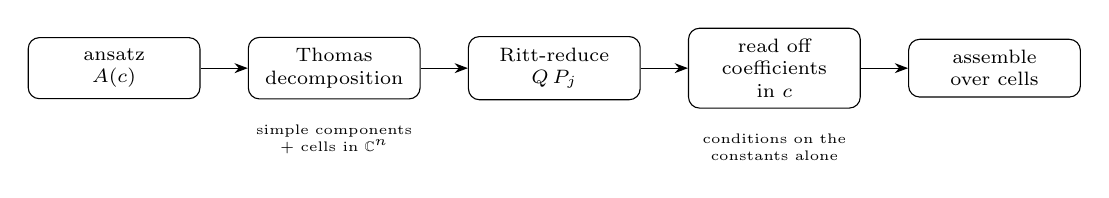
\begin{tikzpicture}[
  node distance=6mm,
  box/.style={draw, rounded corners, align=center, inner sep=4pt,
              text width=19mm, font=\scriptsize},
  >={Stealth[]}
]
\node[box] (a) {ansatz\\$A(c)$};
\node[box, right=of a] (b) {Thomas\\decomposition};
\node[box, right=of b] (c) {Ritt-reduce\\$Q\,P_{j}$};
\node[box, right=of c] (d) {read off\\coefficients\\in $c$};
\node[box, right=of d] (e) {assemble\\over cells};
\draw[->] (a) -- (b);
\draw[->] (b) -- (c);
\draw[->] (c) -- (d);
\draw[->] (d) -- (e);
\node[below=2mm of b, font=\tiny, text width=24mm, align=center]
  {simple components\\ + cells in $\C^{n}$};
\node[below=2mm of d, font=\tiny, text width=24mm, align=center]
  {conditions on the\\ constants alone};
\end{tikzpicture}
\end{center}

\pause
\medskip
Only the first two boxes involve differential algebra. Everything after is
commutative algebra and algebraic geometry in the $n$ constants.
\end{frame}

\begin{frame}{The projection step}
After reducing $Q P_{j}$ modulo a component we have a remainder $r_{j}$. Split
each term into a power product in the \emph{non-constant} indeterminates and a
coefficient in the \emph{constants}:
\[
  r_{j} \;=\; \sum_{\alpha} m_{j\alpha}\; p_{j\alpha}(c) .
\]

\pause
\medskip
Distinct monomials are linearly independent, so
\[
  r_{j}(\cstar) = 0
  \iff
  p_{j\alpha}(\cstar) = 0 \text{ for every } \alpha .
\]

\pause
\medskip
\begin{alertblock}{}
This is the whole projection: \alert{no elimination is required}. The
coefficients already involve nothing but the constants, so they describe a locus
in $\C^{n}$ directly.
\end{alertblock}
\end{frame}

\begin{frame}{Completeness}
\begin{block}{Theorem}
Let $(S^{=},S^{\neq})$ be one simple component of a Thomas decomposition of the
ansatz, with equations $A$ and initials-and-separants product $q$. Reduce each
$Q P_{j}$ modulo $A$, and let
\[
  \mathcal{V} \;=\; V\Bigl( \bigcup_{j} \operatorname{Coeffs}
     \bigl(r_{j},\, \Q[c_{1},\dots,c_{n}]\bigr) \Bigr) .
\]
Then, for $\cstar$ in the component's cell,
\[
  \cstar \in \mathcal{V}
  \iff
  Q P_{j} \in [A(\cstar)] : q^{\infty} \quad (j = 1,\dots,t).
\]
\end{block}

\pause
\medskip
It is an \alert{equivalence}. So the algorithm is complete (nothing valid is
missed) \emph{and} sound (nothing spurious is returned).
\end{frame}

\begin{frame}{Why the proof works}
Reduction gives $h_{j}\cdot Q P_{j} - r_{j} \in [A]$. Specialize at $\cstar$.

\pause
\medskip
\begin{enumerate}
  \item $\cstar$ lies in the cell, so the specialized system is \emph{still
        simple} --- this is where algebraic simplicity (A2), (A3) earn their
        keep, and where $h_{j}(\cstar) \neq 0$ comes from.
  \item $r_{j}(\cstar)$ is fully reduced, hence its own pseudo-remainder. By the
        Proposition, $r_{j}(\cstar) = 0 \iff r_{j}(\cstar) \in E:q^{\infty}$.
  \item $h_{j}$ divides a power of $q$, and $E:q^{\infty}$ is unchanged by further
        saturation at $q$, so $h_{j}$ can be cancelled.
  \item Chaining: $r_{j}(\cstar) = 0 \iff Q P_{j} \in E : q^{\infty}$.
  \item Monomials are independent: $r_{j}(\cstar)=0 \iff$ all coefficients vanish.
\end{enumerate}

\pause
\medskip
Every step is reversible. That is the whole reason the theorem is an equivalence
rather than an implication.
\end{frame}

\begin{frame}{Assembling over the decomposition}
Each component $i$ carries a \alert{cell} $C_{i} \subseteq \C^{n}$ --- the
projection of its solution set --- and a variety $\mathcal{V}_{i}$.

\pause
\medskip
Cells are locally closed, may \alert{overlap}, and need not cover $\C^{n}$.

\pause
\begin{block}{Corollary}
\[
  \cstar \in V_{\forall}
  \iff
  \cstar \in \mathcal{V}_{i} \ \text{ for every $i$ whose cell contains } \cstar .
\]
\end{block}

\pause
\medskip
So: an \alert{intersection} across components, but each component is consulted
only where its own cell lies.

\medskip
No consistency hypothesis is needed --- where the ansatz has no solutions at all,
the radical is the unit ideal and the condition holds vacuously, correctly.
\end{frame}

%% OPTIONAL
\begin{frame}{What comes out}
The output is a \alert{constructible} subset of $\C^{n}$: a finite union of
irreducible locally closed pieces, each presented as a pair
$(\mathfrak{p}, h)$ --- a prime ideal and an inequation.

\pause
\medskip
Not a variety, and not by accident: $V_{\forall}$ is obtained by projecting, and
by Chevalley's theorem projections of constructible sets are constructible, not
closed.

\pause
\medskip
A second, cheaper assembly returns an intermediate locus $V_{\exists\forall}$ with
\[
  V_{\forall} \;\subseteq\; V_{\exists\forall} \;\subseteq\; V_{\exists},
\]
trading exactness for the cost of a union in place of an intersection.
\end{frame}

% ============================================================ PART 5

\section{Examples}

\begin{frame}{Hydrogen: the setup}
\[
  R \;=\; \Q[x,y,z]\{\,\Psi, \Psi', \Psi'', v, r,\;
     E, a_{0}, a_{1}, b_{0}, b_{1}, c_{0}, c_{1}, v_{1}, v_{2}, v_{3}, v_{4}\,\}
\]
with $\Delta = \{\delta_{x},\delta_{y},\delta_{z}\}$.

\pause
\begin{itemize}
  \item $x,y,z$ in the coefficient ring, $\delta_{i}x_{j} = \delta_{ij}$.
  \item Eleven \alert{constants}, killed by every derivation, ranked in the
        lowest block.
  \item Five non-constant differential indeterminates. $r$ carries
        $r^{2}-x^{2}-y^{2}-z^{2}$ as an equation of the system.
\end{itemize}

\pause
\begin{alertblock}{A point worth pausing on}
$E$ is a constant of the \emph{PDE}, not of the ansatz --- but the algorithm makes
no distinction. All eleven are ranked together, so the \alert{eigenvalue is solved
for, not supplied}.
\end{alertblock}
\end{frame}

\begin{frame}{Hydrogen: what the algorithm returns}
The membership locus is a constructible subset of $\C^{11}$, and it has exactly
two components of interest:

\medskip
\begin{columns}[T]
\begin{column}{0.48\textwidth}
$v = r$, the classical branch
\[
  \Psi = e^{-r}, \qquad E = -\tfrac{1}{2}
\]
recovering separation of variables.
\end{column}
\begin{column}{0.48\textwidth}
$v = x+r$, the other branch
\[
  \Psi = J_{0}(2\sqrt{x+r}), \qquad E = 0 .
\]
\end{column}
\end{columns}

\pause
\bigskip
\begin{alertblock}{}
The completeness theorem says these are \alert{all} of them --- within this
ansatz. Not "here are two solutions we found", but "here are the only ones there
are".
\end{alertblock}
\end{frame}

\begin{frame}{Is the new solution physical?}
No --- and the reason is instructive.

\pause
\medskip
A wavefunction must lie in $L^{2}(\mathbb{R}^{3})$. But $J_{0}(0) = 1$ and
$2\sqrt{x+r}$ vanishes along the \emph{entire} negative $x$-axis, so there is a
tube of positive measure and infinite extent on which
$J_{0}(2\sqrt{x+r}) \approx 1$. Hence not square-integrable.

\pause
\medskip
\begin{block}{The failure is structural}
In parabolic coordinates $\xi = r+x$, $\eta = r-x$, our solution depends on $\xi$
alone. That forces the $\eta$ separation constant to vanish, which pins
$E = 0$ --- the threshold between discrete and continuous spectra.
\end{block}

\pause
\medskip
Bound states need \emph{both} parabolic coordinates. A solution that is a function
of one combination $v$ necessarily lands on the non-normalizable threshold.
\end{frame}

%% OPTIONAL
\begin{frame}{Navier--Stokes: a nonlinear system of four}
Incompressible Navier--Stokes: four equations, four dependent variables, and a
genuine nonlinearity in $(\bar{\mathbf{v}}\cdot\nabla)\bar{\mathbf{v}}$.

\pause
\medskip
The machinery runs \alert{unchanged}. What it returns is exactly the
\alert{parallel shear flows} --- and the two reasons it returns nothing more are
structural, not computational:

\pause
\begin{enumerate}
  \item As long as $u,v,w$ are affine in one common ODE element $\Psi$, the
        velocity is a single profile times a fixed direction, and the convective
        term cannot survive incompressibility.
  \item A monomial $\Psi''^{2}$ blocks the viscous term; dropping it, or working
        on the cell $a_{0}=a_{1}=0$ the decomposition hands you anyway, removes
        this one.
\end{enumerate}

\pause
\medskip
\begin{alertblock}{}
A negative answer that says \emph{why}. Reaching an active nonlinearity needs an
ansatz whose components carry \alert{different} ODE elements.
\end{alertblock}
\end{frame}

% ============================================================ PART 6

\section{Where this goes}

\begin{frame}{What is and is not claimed}
\begin{itemize}
  \item \alert{Complementary} to separation of variables: that asks whether a
        solution is a product; this asks whether a solution satisfies a
        structured ODE.
  \item \alert{Complementary} to similarity reduction --- Lie symmetry,
        Clarkson--Kruskal, Bluman--Cole nonclassical symmetries. Those also reduce
        a PDE to an ODE without assuming a product form, but organise around
        symmetries of the equation.
  \item Here the organising principle is the \alert{differential-algebraic
        structure of the ansatz}. No symmetry of the PDE is presupposed.
  \item And the reduction carries a \alert{completeness certificate}.
\end{itemize}

\pause
\bigskip
The bottleneck is the ansatz: choosing one is currently an art.
\end{frame}

\begin{frame}{The real target, and the wall}
The software repository is named \texttt{helium}. The goal is a closed form for
helium's ground state.

\pause
\medskip
Status: a system of \alert{1570 equations} with \alert{1{,}296{,}960 terms},
testing whether helium is reachable from one candidate ansatz.

\pause
\medskip
Attempts to decompose it into minimal associated primes \alert{exhaust 96\,GB of
RAM}. The Gr\"obner engine cannot spill to disk, nor spread across a cluster.

\pause
\bigskip
\begin{alertblock}{}
"Solving helium" is widely regarded as impossible. There is no proof that its
ground state cannot be built from finitely many linear homogeneous ODEs.
\end{alertblock}
\end{frame}

\begin{frame}{Open problems}
\begin{itemize}
  \item \alert{Ansatz selection.} Can one impose $H^{2}(\Omega)$, or other
        function-space conditions, \emph{before} the differential algebra, and let
        that guide the choice?
  \item \alert{The $\forall$/$\exists$ gap.} $V_{\forall}$ is computable,
        $V_{\exists}$ is what one wants. How much is lost, and when?
  \item \alert{What is the relationship} between the constant ideals and the
        function space they describe?
  \item \alert{Scale.} Gr\"obner engines that survive a million terms.
\end{itemize}
\end{frame}

\begin{frame}[standout]
  Thank you
\end{frame}

\appendix

\begin{frame}{Summary}
\begin{enumerate}
  \item Pick an \alert{ansatz}: differential polynomials with undetermined
        constants, describing solutions built from ODEs.
  \item \alert{Decompose} the ansatz once, into differentially simple systems.
  \item \alert{Reduce} each $Q P_{j}$ modulo each component; read off the
        coefficients in the constants.
  \item \alert{Assemble} across cells to get a constructible subset of $\C^{n}$.
  \item The completeness theorem makes step 3 an \alert{equivalence}: the locus is
        exactly right.
\end{enumerate}

\bigskip
And, along the way, a solution to hydrogen that the textbooks do not have.
\end{frame}

\begin{frame}{References}
\footnotesize
\begin{itemize}
  \item J.\,F.~Ritt, \emph{Differential Algebra}, AMS Colloquium Publications
        \textbf{33}, 1950.
  \item E.\,R.~Kolchin, \emph{Differential Algebra and Algebraic Groups},
        Academic Press, 1973.
  \item T.~B\"achler, V.~Gerdt, M.~Lange-Hegermann, D.~Robertz,
        \emph{Thomas decomposition of algebraic and differential systems},
        J.~Symbolic Comput.\ \textbf{47} (2012) 1233--1266.
  \item D.~Robertz, \emph{Formal Algorithmic Elimination for PDEs}, Lecture Notes
        in Mathematics \textbf{2121}, Springer, 2014.
  \item F.~Boulier, D.~Lazard, F.~Ollivier, M.~Petitot, \emph{Computing
        representations for radicals of finitely generated differential ideals},
        AAECC \textbf{20} (2009) 73--121.
  \item P.~Gianni, B.~Trager, G.~Zacharias, \emph{Gr\"obner bases and primary
        decomposition of polynomial ideals}, J.~Symb.\ Comput.\ \textbf{6} (1988)
        149--167.
\end{itemize}
\end{frame}

\end{document}
